\chapter{Results}
\label{ch:results}

This project classifies bookings from a dataset in the student accommodation industry as either cancelled or not cancelled using a machine learning model with both sklearn and Azure ML. The aim of this study is to produce a prediction probability for each booking, allowing for data-driven decisions to be made with the hope to use the prediction to reduce cancellations. 
\section{Exploratory data analysis}
 \begin{figure}[H]
 %\centering
 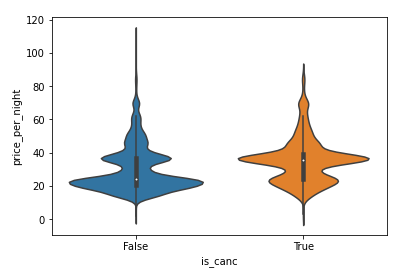
\includegraphics[width=5cm]{figures/price_per_night.png}
 \caption{Distribution of price per night comparing cancelled and non cancelled bookings}
\end{figure}
 
 
 Figure 4.1 shows comparing price per night when looking at bookings that canceled to ones that didn't we can see that the mean price range of £40 per night is where the most significant number of booking cancellations occur, with most of the non canceled bookings in the £20 per night price range. This difference in price distribution when comparing cancelled to non cancelled bookings suggests price per night is an important feature for classification. 
 
\begin{itemize}
\item Could also perform statistical test to comapre difference, something like kruskal wallis test would be good here
\end{itemize}

 
 \begin{figure}[H]
 %\centering
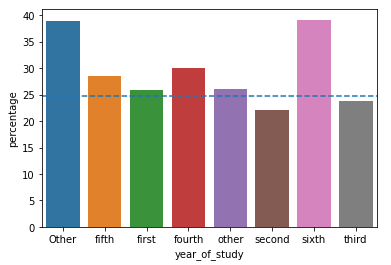
\includegraphics[width=5cm]{figures/canc_per_year.png}
 \caption{Normalized percentage of booking cancellation for degree year of study with blue horizontal line being the mean}
\end{figure}
 
  
Figure 4.2 shows percentage of booking cancellations grouped by academic year of study. This shows sixth years, having 40 percent cancellation this many be due to the fact they are more likely to decide to live in private accommodation but it is unlikely this accounts for them being almost twice as likely to cancel than the average. The Other category is also an outlier here with an almost 40 percent chance of cancelling, more research would be needed to understand exactly why customers who don't enter a year of study are more likely to cancel but it is clear from this figure that year of study will be a good indicator of cancellations.

\vspace{5mm}
  
  \begin{figure}[H]
 %\centering
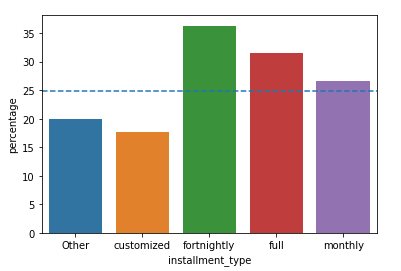
\includegraphics[width=5cm]{figures/instalment_type.png}
 \caption{Normalized percentage of booking cancellation for payment installment type}
\end{figure}
  
  
 Figure 4.3 shows Weighted average of cancellations looking at the selected instalment type. Instalment type is the payment plan the student selected, we can see that students who selected the fortnightly plan are 10 percent more likely to cancel than the average and students who opted for the customized installment plan are around 6 percent less likely to cancel. this may be a good predictor of cancellations.
  
  
   \begin{figure}[H]
 %\centering
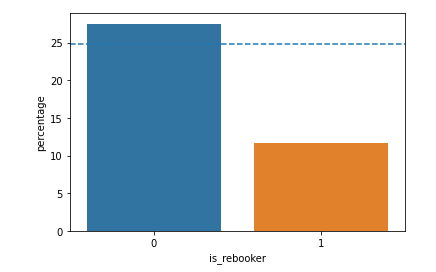
\includegraphics[width=5cm]{figures/is_rebooker.png}
 \caption{Normalized percentage of booking cancellation for rebooker}
\end{figure}
  
 Comparison in cancellations with students who are rebookers (have booked before), we can see that students who have booked previously are around half as likely to cancel there bookings. this is another good predictor of cancellations.  
 
 \section{Original Model - XGBoost}

XGBoost is a distributed gradient boosting library that has been optimised for performance, flexibility, and portability. It uses the Gradient Boosting framework to implement machine learning algorithms. XGBoost is a parallel tree boosting algorithm that solves a variety of data science problems quickly and accurately. XGBoost is commonly used by data scientists to produce cutting-edge performance on a variety of machine learning problems. Various interfaces are supported by XGBoost, including the python interface. The implementation of XGBoost focuses on computational speed, model performance and memory resources.The most critical element in XGBoost's performance is its scalability in all situations. On a single machine, the device is more than ten times faster than current common solutions, and it scales to billions of examples in distributed or memory-limited environments\cite{ChenXGBoost:System}.

 \begin{figure}[H]
 %\centering
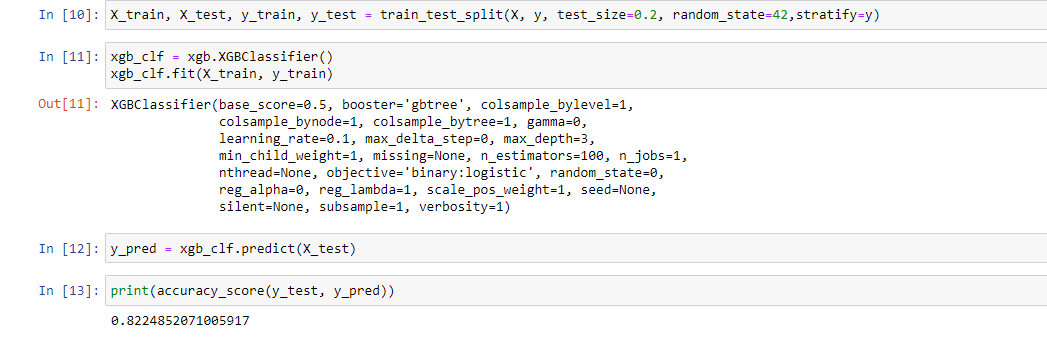
\includegraphics[width=10cm]{figures/xg_boost_code.png}
 \caption{}
\end{figure}

The original methodology included using Python to run XGBoost, Figure shows a snippet of the code used to train the model with a train test split set to 20 percent. The model was created on the test data and the accuracy score was calculated. The model was run using the default hyper parameters, sklearn. Initially, the accuracy score of 82 percent appeared to solve the problem specification. However, the confusion matrix identified that there is a large number of false positive predictions compared with the number of true positive predictions, suggesting that the models recall is low compared to the accuracy. As recall identifies the number of true positives, correct cancellations, a low recall score is undesirable.

 \begin{figure}[H]
 %\centering
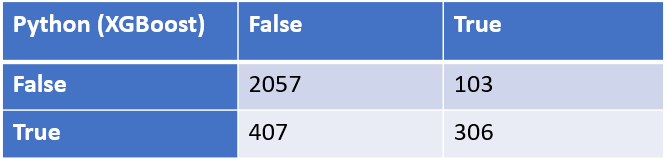
\includegraphics[width=10cm]{figures/python_xgboost.png}
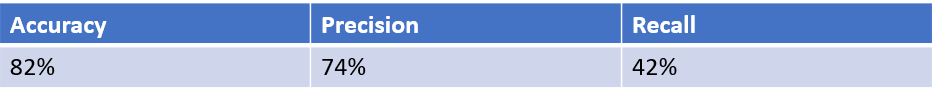
\includegraphics[width=10cm]{figures/python_recall}
 \caption{}
\end{figure}

A confusion matrix is a table that shows how well a classification model performs on a collection of test data for which the true values are known. The 4 sections that make up a confusion matrix are, true positives (TP) these are bookings that the model predicted as cancelled and are actually cancelled. True negatives (TN) these are bookings predicted correctly as not cancelled. False positives (FP) are bookings that the model predicted as cancelled but didn't and False negatives (FN) these are bookings the model predicted as not cancelled but did cancel. TP is the most important because this is where the model has predicted a booking as going  to cancel and has actually cancelled which is the objective of this research.

After running this model and identifying poor recall, a alternative model and hyper parameter combinations needed to be identified to produce increase recall. Using azure ml, different algorithms were tested to enable the best algorithm to be identified. 

\section{Azure ML}
Since AzureML is automated, it allows for more effective testing and evaluation of different models and hyper parameter combinations. This addresses the previous issue of not knowing which model and hyper parameter combination to use in order to solve this problem.

\begin{figure}[H]
 %\centering
 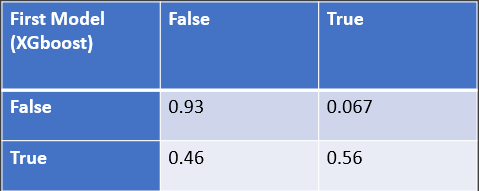
\includegraphics[width=10cm]{figures/xgboost_confusion_matrix.png}
 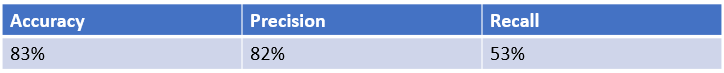
\includegraphics[width=10cm]{figures/original_results.png}
 \caption{Confusion matrix from first run normalized}
\end{figure}

The accuracy of a classification model is (TP+TN)/total. This is the number of bookings accurately classified as either cancelled or not cancelled. In this case it is more valuable to classify TP than TN since cancelled bookings are the focus of this research. Figure \textbf{4.1} shows  0.93TF 0.56TP gives an overall accuracy of 0.83, this appears to be a very good result with over 80 percent of the bookings accurately predicted.

Recall is TP / (TP + FN), this is the proportion of actual positive values predicted correctly \textbf{figure 4.1} showing only 53 percent of true positive values are identified correctly in the first run of azureML. This shows that accuracy is not the most important metric here since even with a good accuracy score, the recall score is very low, with few true positive values predicted, the original problem statement has not been solved. 

\section{Azure ML- Stack Ensemble}

 \begin{figure}[H]
 %\centering
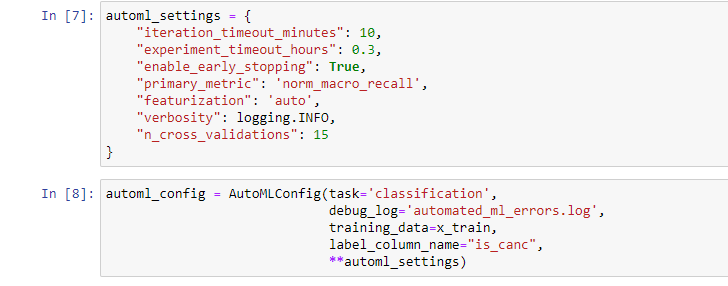
\includegraphics[width=10cm]{figures/auto_ml_settings.png}
 \caption{}
\end{figure}

Knowing that Recall should be my primary metric to target and not accuracy, using Azure ML, the target metric was changed to Recall. \textbf{Figure 4.7} shows the settings applied with the new primary metric being normalized macro recall. Setting the primary metric means Auto ML can optimise the model selection based on recall.

 \begin{figure}[H]
 %\centering
\includegraphics[width=10cm]{figures/auto_ml_final_models.png}
 \caption{}
\end{figure}

During this run I used Azure ML to evaluate and compare multiple different algorithms knowing that I wanted to take the algorithm with the best recall I run Azure ML again keeping all other values the same, and only changing the primary metric. Azure ML performs 15 different cross-validations on the data set, ranking them by the target attribute, recall. The same dataset and train test split were used but the target metric changed to recall,  meaning the model evaluates and ranks the results differently.

When working with many machine learning algorithms, data scaling is a suggested pre-processing stage. Real-valued input and output variables may be normalised or standardised to achieve data scaling. Stack Ensemble uses normalization  to scale each input variable independently to the range 0-1.  This estimator scales and translates each feature separately, resulting in a maximum absolute value of 1.0 for each feature in the training set. It does not shift or centre the data, so there is no loss of sparsity \cite{Singh2019MLlib:Library,Sklearn.preprocessing.MaxAbsScalerDocumentation}



\begin{figure}[H]
 %\centering
 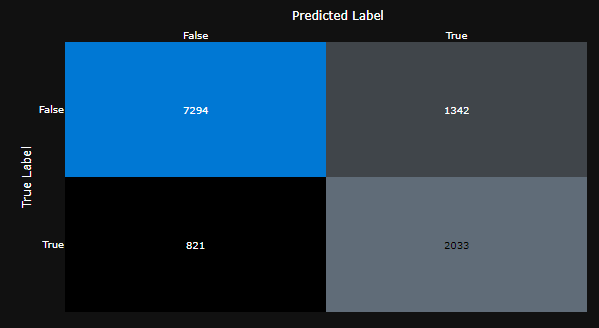
\includegraphics[width=10cm]{figures/azure_ml_confusion_matrix.png}
 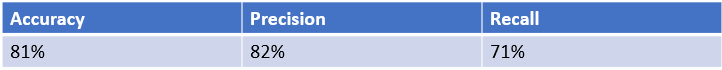
\includegraphics[width=10cm]{figures/final_recall.png}
 \caption{Confusion matrix from final run of StackEnsemble algorithm, shows 71 percent recall}
\end{figure}
The confusion matrix in figure 4.9 shows a significant improvement when compared to the confusion matrix in figure 4.6. This outlines the benefit of using the Stack Ensemble algorithm compared to XGBoost. Stack Ensemble learns how to integrate the predictions from two or more base machine learning algorithms using a meta-learning algorithm. The advantage of stacking is that it can combine the capabilities of a number of high-performing models to make predictions that outperform any single model in the ensemble on a classification. This is made up from 2 or more base models and a meta model that combines the predictions of the base models.

In comparison to Figure 4.6, the final confusion matrix has a lower overall accuracy score but a higher recall score. There is a trade-off between having a high accuracy and a high recall score. However, as the recall is a representation of the true predicted cancellations, a higher recall score is more desirable. The final model had a recall score of 71 percent (Figure 4.9) which is around 20 percent higher than the original model. 

\begin{figure}[H]
 %\centering
 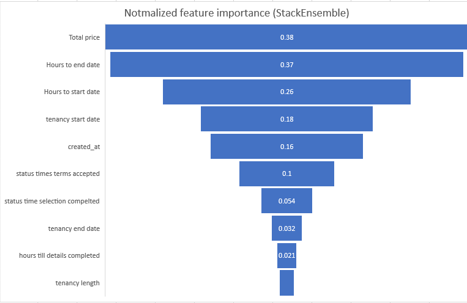
\includegraphics[width=10cm]{figures/feature_importance.png}
 \caption{}
\end{figure}

Price per night= total price. top importance on this graph and important in feature explanation
largely numerical features, unexpected

Based on the results from the feature importance graph in Figure..., the main dependent feature on cancellations was total price This was consistent with the feature exploration graph in Figure 4.1 which indicated price per night to be the most important feature. However, the rest of the features indicated in the exploratory data analysis were not present in the feature importance graph in Figure...The majority of the features in the feature importance graph were based on numerical data, such as hours to end or start date. 


\begin{figure}[H]
 %\centering
 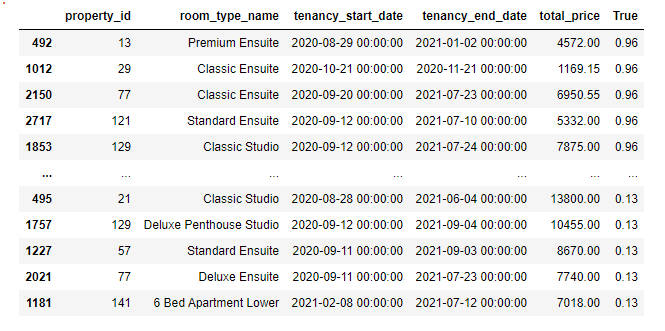
\includegraphics[width=10cm]{figures/canc_prob.png}
 \caption{prediction probability ranking each of the bookings made a chance of canceling}
\end{figure}
All of the bookings in the test data are ranked between 0 and 1, over 0.5 booking gets classified as cancelled. The prediction probability was calculated using the Stack Ensemble model and is able to rank bookings made by the chance of them being cancelled. The implementation of the predictions into the booking management system is indicated in Figure 4.11, illustrating that the problem statement has been solved and Incorporated in a useful way. 



